\section{mo\-TSMove\-Loop\-Expl$<$ M $>$ Class Template Reference}
\label{classmo_t_s_move_loop_expl}\index{moTSMoveLoopExpl@{moTSMoveLoopExpl}}
Explorer for a Tabu Search algorithm.  


{\tt \#include $<$mo\-TSMove\-Loop\-Expl.h$>$}

Inheritance diagram for mo\-TSMove\-Loop\-Expl$<$ M $>$::\begin{figure}[H]
\begin{center}
\leavevmode
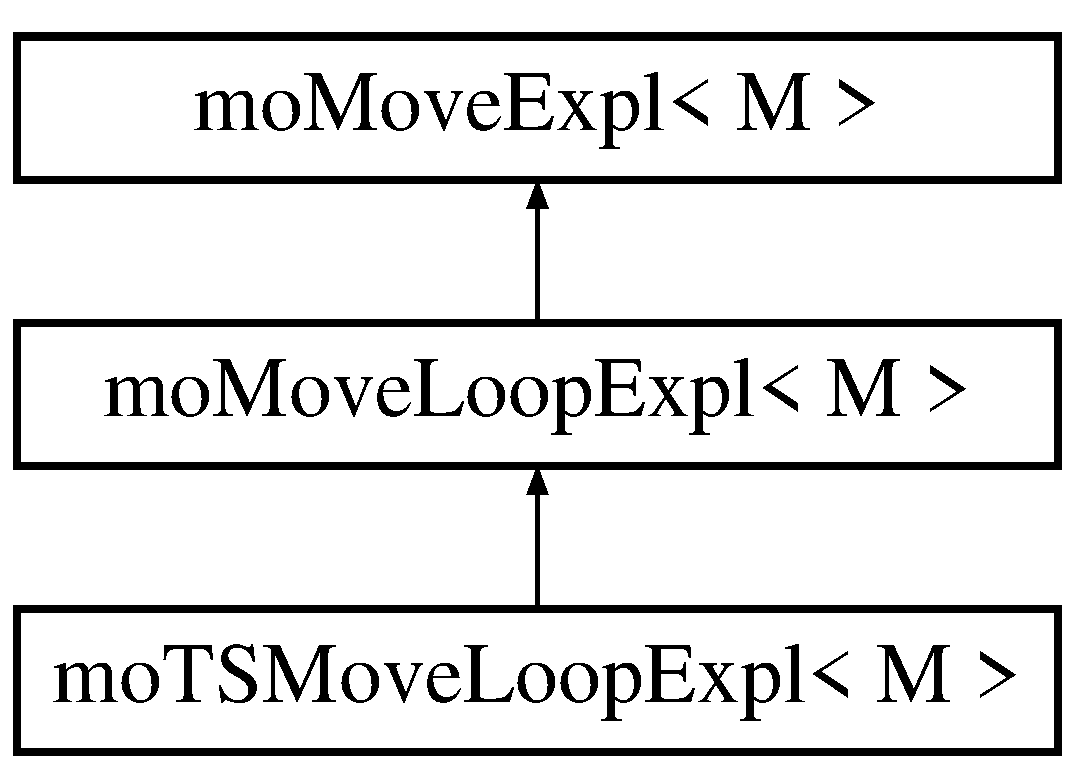
\includegraphics[height=5cm]{classmo_t_s_move_loop_expl}
\end{center}
\end{figure}
\subsection*{Public Member Functions}
\begin{CompactItemize}
\item 
{\bf mo\-TSMove\-Loop\-Expl} ({\bf mo\-Move\-Init}$<$ M $>$ \&\_\-move\_\-initializer, {\bf mo\-Next\-Move}$<$ M $>$ \&\_\-next\_\-move\_\-generator, {\bf mo\-Move\-Incr\-Eval}$<$ M $>$ \&\_\-incremental\_\-evaluation, {\bf mo\-Tabu\-List}$<$ M $>$ \&\_\-tabu\_\-list, {\bf mo\-Aspir\-Crit}$<$ M $>$ \&\_\-aspiration\_\-criterion)
\begin{CompactList}\small\item\em Constructor. \item\end{CompactList}\item 
void {\bf operator()} (const {\bf EOT} \&\_\-old\_\-solution, {\bf EOT} \&\_\-new\_\-solution)
\begin{CompactList}\small\item\em Procedure which lauches the exploration. \item\end{CompactList}\end{CompactItemize}
\subsection*{Private Types}
\begin{CompactItemize}
\item 
typedef M::EOType {\bf EOT}\label{classmo_t_s_move_loop_expl_y0}

\begin{CompactList}\small\item\em Alias for the type. \item\end{CompactList}\item 
typedef M::EOType::Fitness {\bf Fitness}\label{classmo_t_s_move_loop_expl_y1}

\begin{CompactList}\small\item\em Alias for the fitness. \item\end{CompactList}\end{CompactItemize}
\subsection*{Private Attributes}
\begin{CompactItemize}
\item 
{\bf mo\-Move\-Init}$<$ M $>$ \& {\bf move\_\-initializer}\label{classmo_t_s_move_loop_expl_r0}

\begin{CompactList}\small\item\em Move initialisation. \item\end{CompactList}\item 
{\bf mo\-Next\-Move}$<$ M $>$ \& {\bf next\_\-move\_\-generator}\label{classmo_t_s_move_loop_expl_r1}

\begin{CompactList}\small\item\em Neighborhood explorer. \item\end{CompactList}\item 
{\bf mo\-Move\-Incr\-Eval}$<$ M $>$ \& {\bf incremental\_\-evaluation}\label{classmo_t_s_move_loop_expl_r2}

\begin{CompactList}\small\item\em Efficient evaluation. \item\end{CompactList}\item 
{\bf mo\-Best\-Impr\-Select}$<$ M $>$ {\bf move\_\-selection}\label{classmo_t_s_move_loop_expl_r3}

\begin{CompactList}\small\item\em Move selector. \item\end{CompactList}\item 
{\bf mo\-Tabu\-List}$<$ M $>$ \& {\bf tabu\_\-list}\label{classmo_t_s_move_loop_expl_r4}

\begin{CompactList}\small\item\em Tabu list. \item\end{CompactList}\item 
{\bf mo\-Aspir\-Crit}$<$ M $>$ \& {\bf aspiration\_\-criterion}\label{classmo_t_s_move_loop_expl_r5}

\begin{CompactList}\small\item\em Aspiration criterion. \item\end{CompactList}\end{CompactItemize}


\subsection{Detailed Description}
\subsubsection*{template$<$class M$>$ class mo\-TSMove\-Loop\-Expl$<$ M $>$}

Explorer for a Tabu Search algorithm. 

It is used by a {\bf mo\-TS}{\rm (p.\,\pageref{classmo_t_s})}. 



Definition at line 53 of file mo\-TSMove\-Loop\-Expl.h.

\subsection{Constructor \& Destructor Documentation}
\index{moTSMoveLoopExpl@{mo\-TSMove\-Loop\-Expl}!moTSMoveLoopExpl@{moTSMoveLoopExpl}}
\index{moTSMoveLoopExpl@{moTSMoveLoopExpl}!moTSMoveLoopExpl@{mo\-TSMove\-Loop\-Expl}}
\subsubsection{\setlength{\rightskip}{0pt plus 5cm}template$<$class M$>$ {\bf mo\-TSMove\-Loop\-Expl}$<$ M $>$::{\bf mo\-TSMove\-Loop\-Expl} ({\bf mo\-Move\-Init}$<$ M $>$ \& {\em \_\-move\_\-initializer}, {\bf mo\-Next\-Move}$<$ M $>$ \& {\em \_\-next\_\-move\_\-generator}, {\bf mo\-Move\-Incr\-Eval}$<$ M $>$ \& {\em \_\-incremental\_\-evaluation}, {\bf mo\-Tabu\-List}$<$ M $>$ \& {\em \_\-tabu\_\-list}, {\bf mo\-Aspir\-Crit}$<$ M $>$ \& {\em \_\-aspiration\_\-criterion})\hspace{0.3cm}{\tt  [inline]}}\label{classmo_t_s_move_loop_expl_a0}


Constructor. 

\begin{Desc}
\item[Parameters:]
\begin{description}
\item[{\em \_\-move\_\-initializer}]The move initializer. \item[{\em \_\-next\_\-move\_\-generator}]The neighbourhood explorer. \item[{\em \_\-incremental\_\-evaluation}]A (generally) efficient evaluation. \item[{\em \_\-tabu\_\-list}]The tabu list. \item[{\em \_\-aspiration\_\-criterion}]An aspiration criterion. \end{description}
\end{Desc}


Definition at line 71 of file mo\-TSMove\-Loop\-Expl.h.

References mo\-TSMove\-Loop\-Expl$<$ M $>$::aspiration\_\-criterion, mo\-TSMove\-Loop\-Expl$<$ M $>$::incremental\_\-evaluation, mo\-TSMove\-Loop\-Expl$<$ M $>$::move\_\-initializer, mo\-TSMove\-Loop\-Expl$<$ M $>$::next\_\-move\_\-generator, and mo\-TSMove\-Loop\-Expl$<$ M $>$::tabu\_\-list.

\subsection{Member Function Documentation}
\index{moTSMoveLoopExpl@{mo\-TSMove\-Loop\-Expl}!operator()@{operator()}}
\index{operator()@{operator()}!moTSMoveLoopExpl@{mo\-TSMove\-Loop\-Expl}}
\subsubsection{\setlength{\rightskip}{0pt plus 5cm}template$<$class M$>$ void {\bf mo\-TSMove\-Loop\-Expl}$<$ M $>$::operator() (const {\bf EOT} \& {\em \_\-old\_\-solution}, {\bf EOT} \& {\em \_\-new\_\-solution})\hspace{0.3cm}{\tt  [inline]}}\label{classmo_t_s_move_loop_expl_a1}


Procedure which lauches the exploration. 

The exploration continues while the chosen move is not in the tabu list or the aspiration criterion is true. If these 2 conditions are not true, the exploration stops if the move selector update function returns false.

\begin{Desc}
\item[Parameters:]
\begin{description}
\item[{\em \_\-old\_\-solution}]the initial solution \item[{\em \_\-new\_\-solution}]the new solution \end{description}
\end{Desc}


Definition at line 90 of file mo\-TSMove\-Loop\-Expl.h.

References mo\-TSMove\-Loop\-Expl$<$ M $>$::aspiration\_\-criterion, mo\-TSMove\-Loop\-Expl$<$ M $>$::Fitness, mo\-TSMove\-Loop\-Expl$<$ M $>$::incremental\_\-evaluation, mo\-TSMove\-Loop\-Expl$<$ M $>$::move\_\-initializer, mo\-TSMove\-Loop\-Expl$<$ M $>$::move\_\-selection, mo\-TSMove\-Loop\-Expl$<$ M $>$::next\_\-move\_\-generator, and mo\-TSMove\-Loop\-Expl$<$ M $>$::tabu\_\-list.

The documentation for this class was generated from the following file:\begin{CompactItemize}
\item 
mo\-TSMove\-Loop\-Expl.h\end{CompactItemize}
